
\documentclass{article}
\usepackage[utf8]{inputenc}

\title{Laboratorio01_CALIDAD_PRUEBAS_SOFTWARE}
\author{edwartbalcon }
\date{October 2020}

\usepackage[utf8]{inputenc}
\usepackage[spanish]{babel}
\usepackage{natbib}
\usepackage{graphicx}

\begin{document}

\title{Caratula}

\begin{titlepage}
\begin{center}
\begin{Large}
\textbf{UNIVERSIDAD PRIVADA DE TACNA} \\
\end{Large}
\vspace*{-0.025in}
\begin{figure}[htb]
\begin{center}

\includegraphics[width=6cm]{./images/logo_UPT}
\end{center}
\end{figure}
\vspace*{-0.025in}
\begin{Large}
\textbf{FACULTAD DE INGENIERIA} \\
\end{Large}
\vspace*{0.05in}
\begin{Large}
\textbf{Escuela Profesional de Ingeniería de Sistema} \\
\end{Large}


\vspace*{0.4in}

\vspace*{0.1in}
\begin{Large}
\textbf{Informe de laboratorio 01} \\
\end{Large}

\vspace*{0.3in}
\begin{Large}
\textbf{Curso: Calidad y Pruebas de Software} \\
\end{Large}

\vspace*{0.3in}
\begin{Large}
\textbf{DOCENTE: Ing. Patrick Cuadros Quiroga} \\
\end{Large}

\vspace*{0.2in}
\vspace*{0.1in}
\begin{large}

\begin{Large}
\textbf{Alumno: Balcon Coahila, Edwart Juan\hfill	(2013046516) } \\
\end{Large}

\vspace*{0.15in}
\begin{Large}
\textbf{Tacna – Perú} \\
\end{Large}

\vspace*{0.05in}
\begin{Large}
\textbf{2020 } \\
\end{Large}

\end{large}
\end{center}

\end{titlepage}


\newpage


\textbf{1.Descargar SonarQube}

    \begin{center}
		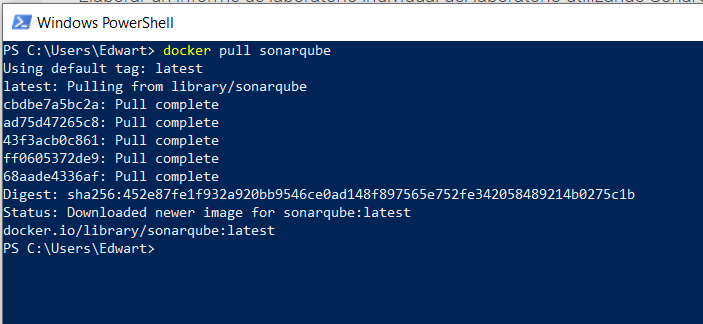
\includegraphics[width=15cm]{./images/1} 
	\end{center}

\textbf{2. Ejecutar una instancia de SonarQube}

    \begin{center}
		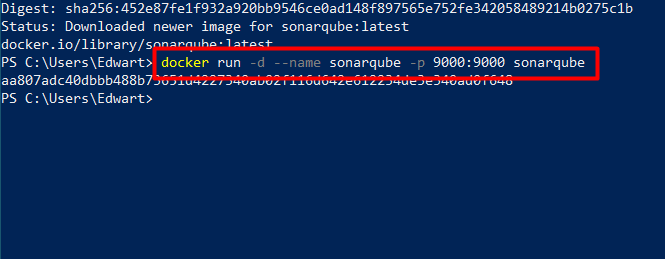
\includegraphics[width=15cm]{./images/2} 
	\end{center}
  
  \newpage
\textbf{3.Ingresar al portal con las credenciales}

    \begin{center}
		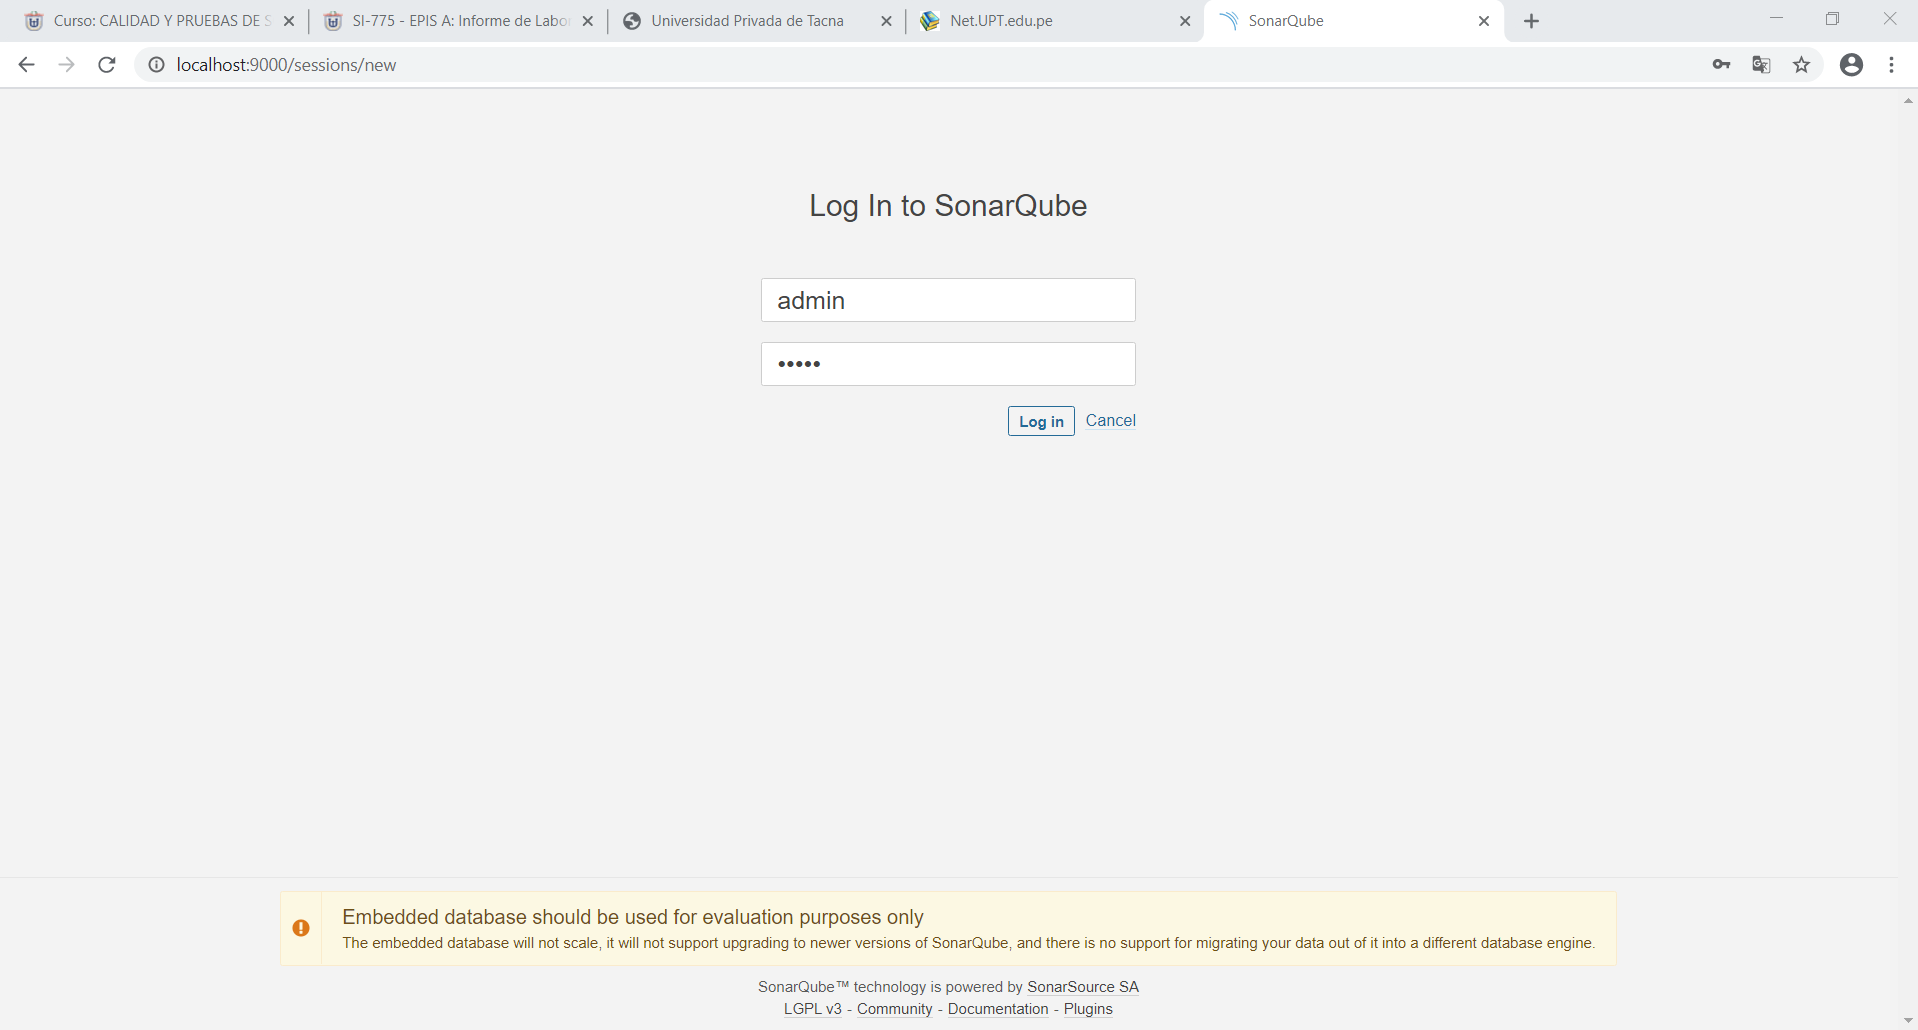
\includegraphics[width=15cm]{./images/3} 
	\end{center}
\newpage
\textbf{4. Crear una nueva aplicación con el nombre aplicacionNetCore}

    \begin{center}
		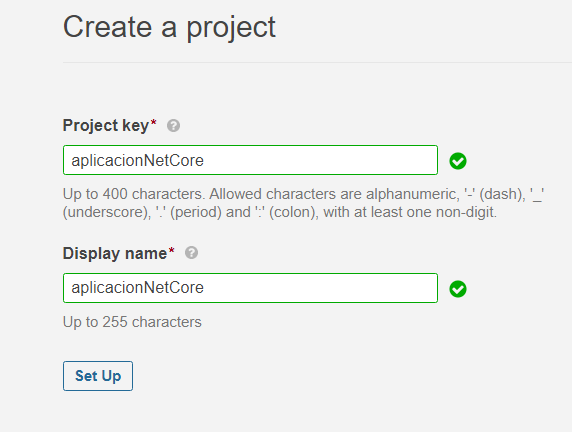
\includegraphics[width=15cm]{./images/4} 
	\end{center}
	
\newpage

\textbf{5.Generar el token de la nueva aplicación aplicacionNetCore, debera devolver algo similar a 8a15d2a89c8636f15eb32ebee0993b8d16bff94e}

    \begin{center}
		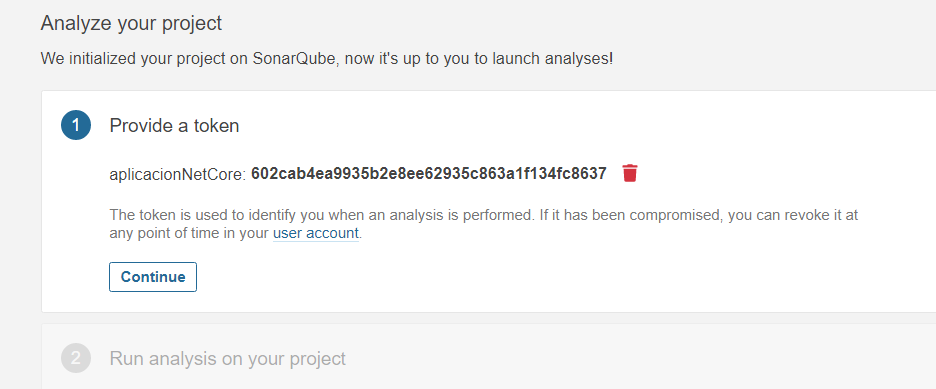
\includegraphics[width=15cm]{./images/5} 
	\end{center}
	
\newpage
\textbf{6. Descargar Net Core e instalar}

    \begin{center}
		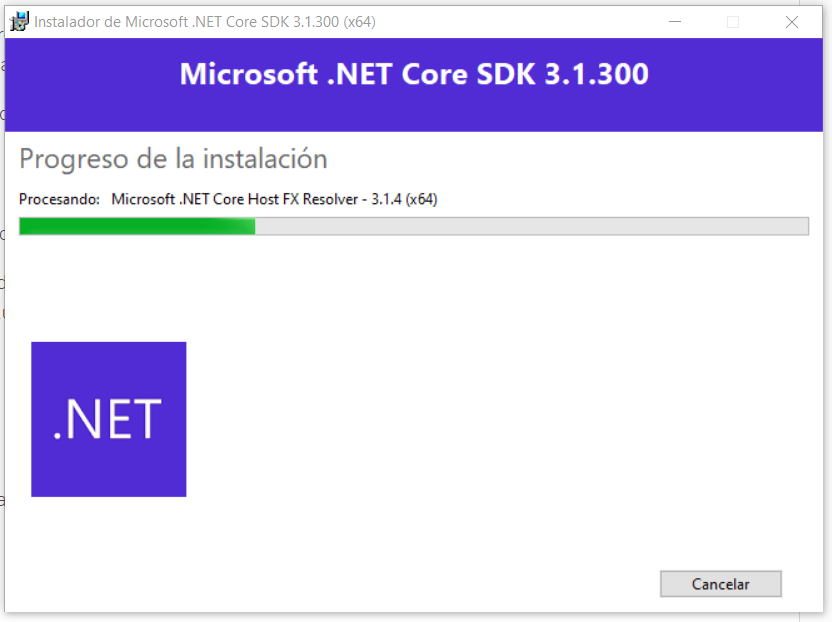
\includegraphics[width=15cm]{./images/6} 
	\end{center}

\textbf{7. En un terminal ejecutar e instalar sonar-scanner}

    \begin{center}
		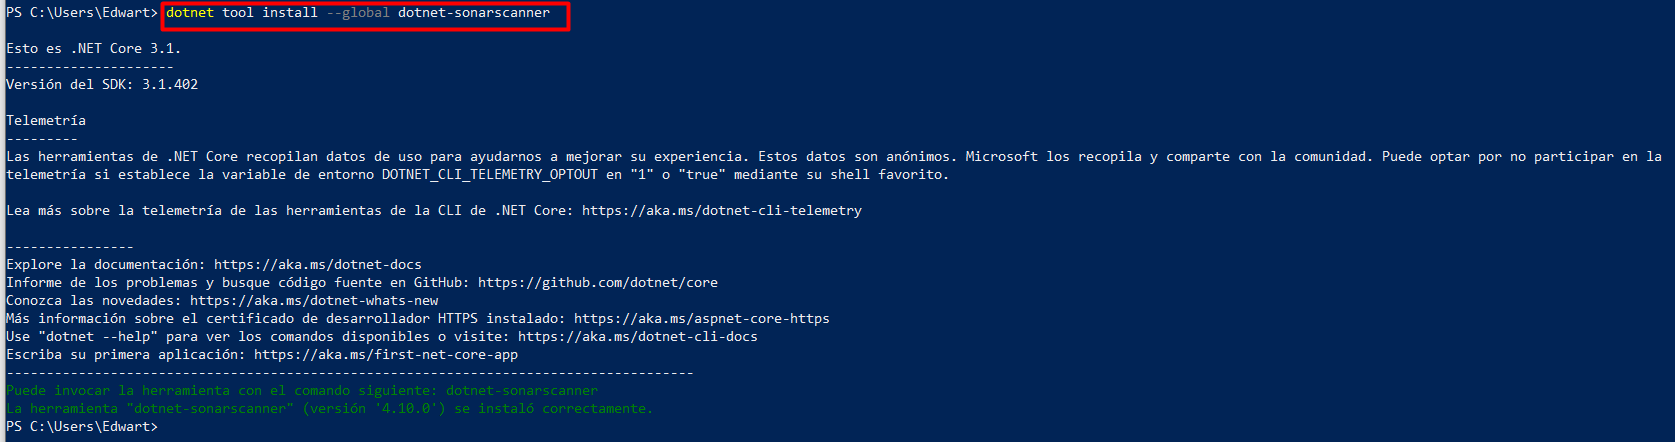
\includegraphics[width=15cm]{./images/7} 
	\end{center}
\newpage
\textbf{8. En un terminal, acceder a una ruta donde creara una nueva aplicación}

    \begin{center}
		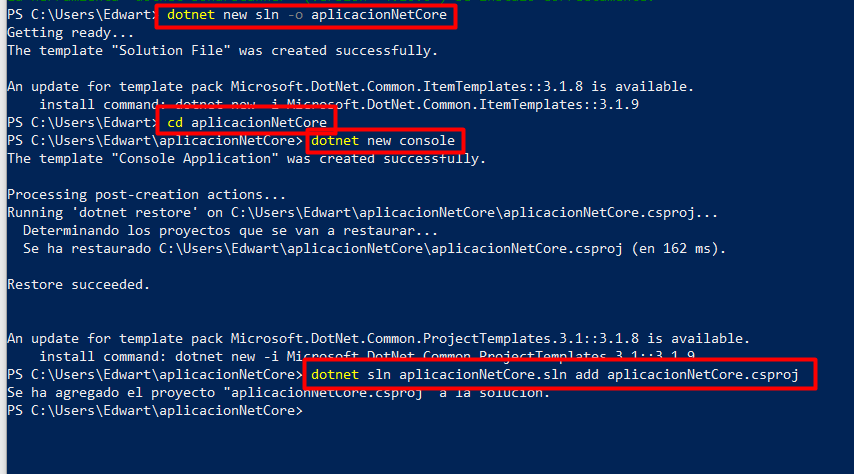
\includegraphics[width=15cm]{./images/8} 
	\end{center}
	


\textbf{9. En el mismo terminal, iniciar la sesión de revisión de sonarqube}

   \begin{center}
		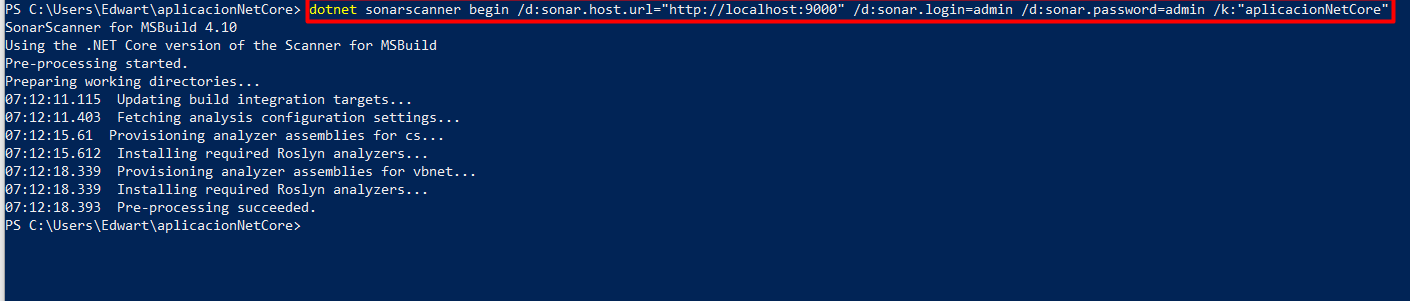
\includegraphics[width=15cm]{./images/9} 
	\end{center}


\textbf{10. Compilar la aplicación}

    \begin{center}
		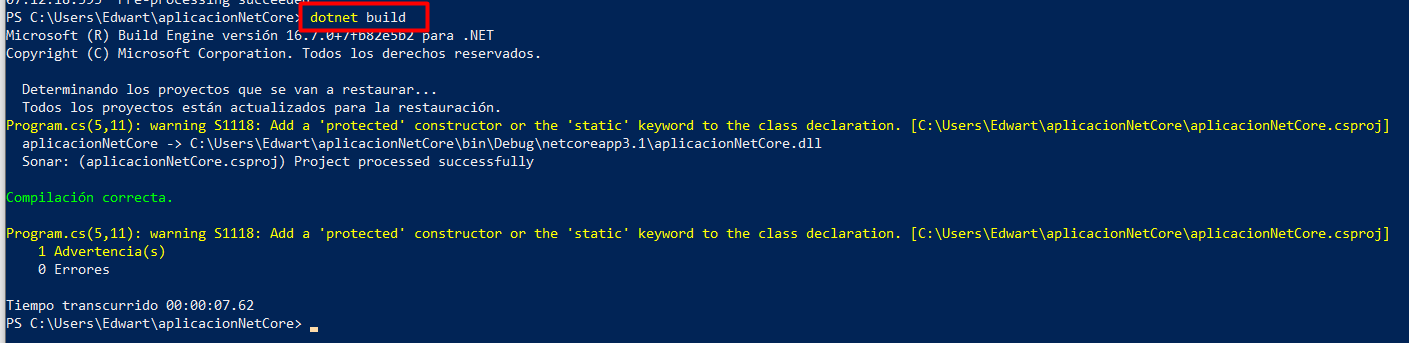
\includegraphics[width=15cm]{./images/10} 
	\end{center}
	
	
\textbf{11. Cerramos la sesión}

    \begin{center}
		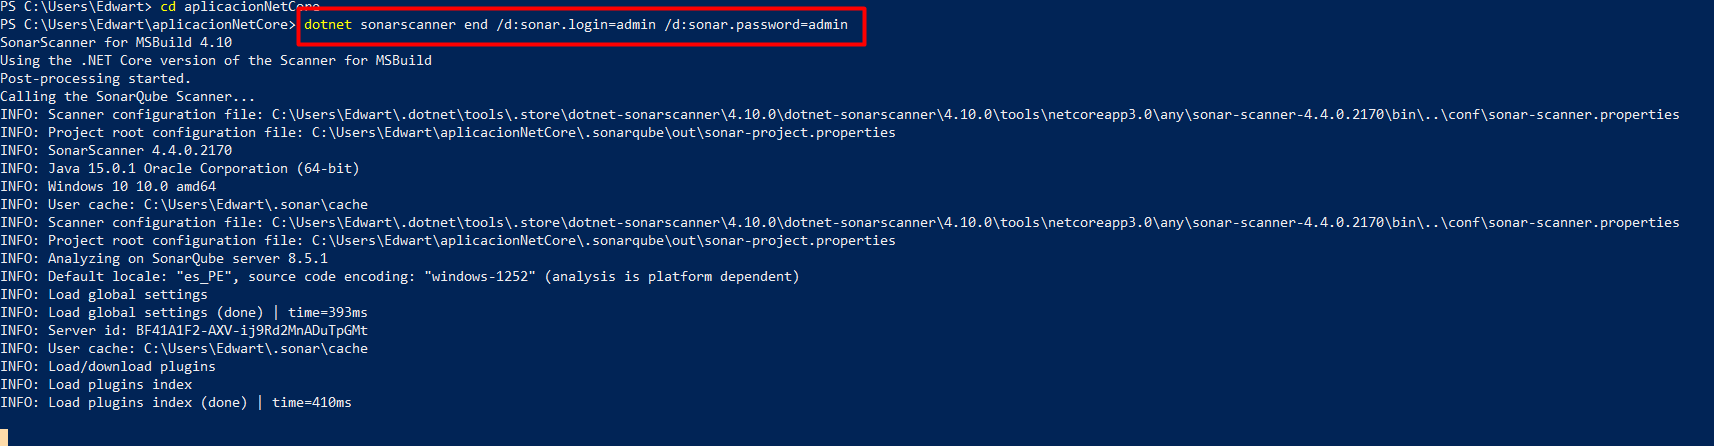
\includegraphics[width=15cm]{./images/11} 
	\end{center}


   
\end{document}
